\documentclass[13pt,a4paper]{article}
\usepackage{a4wide,amssymb,epsfig,latexsym,multicol,array,hhline,fancyhdr}
\usepackage{vntex}
\usepackage{amsmath}
\usepackage{lastpage}
\usepackage[lined,boxed,commentsnumbered]{algorithm2e}
\usepackage{enumerate}
\usepackage{color}
\usepackage{graphicx}							% Standard graphics package
\usepackage{array}
\usepackage{tabularx, caption}
\usepackage{multirow}
\usepackage{multicol}
\usepackage{rotating}
\usepackage{graphics}
\usepackage{geometry}
\usepackage{setspace}
\usepackage{epsfig}
\usepackage{tikz}
\usetikzlibrary{arrows,snakes,backgrounds}
\usepackage{hyperref}
\hypersetup{urlcolor=blue,linkcolor=black,citecolor=black,colorlinks=true} 
%\usepackage{pstcol} 								% PSTricks with the standard color package

\newtheorem{theorem}{{\bf Theorem}}
\newtheorem{property}{{\bf Property}}
\newtheorem{proposition}{{\bf Proposition}}
\newtheorem{corollary}[proposition]{{\bf Corollary}}
\newtheorem{lemma}[proposition]{{\bf Lemma}}

\AtBeginDocument{\renewcommand*\contentsname{Contents}}
\AtBeginDocument{\renewcommand*\refname{References}}
%\usepackage{fancyhdr}
\setlength{\headheight}{40pt}
\pagestyle{fancy}
\fancyhead{} % clear all header fields
\fancyhead[L]{
	\begin{tabular}{rl}
		\begin{picture}(25,15)(0,0)
			\put(0,-8){
\includegraphics[width=8mm, height=8mm]{hcmut.png}}
			%\put(0,-8){\epsfig{width=10mm,figure=hcmut.eps}}
		\end{picture}&
		%
\includegraphics[width=8mm, height=8mm]{hcmut.png} & %
		\begin{tabular}{l}
			\textbf{\bf \ttfamily University of Technology, Ho Chi Minh City}\\
			\textbf{\bf \ttfamily Faculty of Computer Science and Engineering}
		\end{tabular} 	
	\end{tabular}
}
\fancyhead[R]{
	\begin{tabular}{l}
		\tiny \bf \\
		\tiny \bf 
\end{tabular}  }
\fancyfoot{} % clear all footer fields
\fancyfoot[L]{\scriptsize \ttfamily Lab 7 for Operating Systems year 2020 - 2021}
\fancyfoot[R]{\scriptsize \ttfamily Page {\thepage}/\pageref{LastPage}}
\renewcommand{\headrulewidth}{0.3pt}
\renewcommand{\footrulewidth}{0.3pt}


%%%
\setcounter{secnumdepth}{4}
\setcounter{tocdepth}{3}
\makeatletter
\newcounter {subsubsubsection}[subsubsection]
\renewcommand\thesubsubsubsection{\thesubsubsection .\@alph\c@subsubsubsection}
\newcommand\subsubsubsection{\@startsection{subsubsubsection}{4}{\z@}%
	{-3.25ex\@plus -1ex \@minus -.2ex}%
	{1.5ex \@plus .2ex}%
	{\normalfont\normalsize\bfseries}}
\newcommand*\l@subsubsubsection{\@dottedtocline{3}{10.0em}{4.1em}}
\newcommand*{\subsubsubsectionmark}[1]{}
\makeatother

\begin{document}
	
	\begin{titlepage}
		\begin{center}
			VIETNAM NATIONAL UNIVERSITY, HO CHI MINH CITY \\
			UNIVERSITY OF TECHNOLOGY \\
			FACULTY OF COMPUTER SCIENCE AND ENGINEERING
		\end{center}
		
		\vspace{1cm}
		
		\begin{figure}[h!]
			\begin{center}
				
\includegraphics[width=3cm]{hcmut.png}
			\end{center}
		\end{figure}
		
		\vspace{1cm}
		
		\begin{center}
			\color{blue}
			\begin{tabular}{c}
				\multicolumn{1}{l}{\textbf{\centerline{{\Huge OPERATING SYSTEMS}}}}\\
				~~\\
				\hline
				\\
				\multicolumn{1}{l}{\textbf{\centerline{{\LARGE Report \#07}}}}\\
				\\
				\textbf{{\Huge Lab 07 : Scheduling}}\\
				\\
				\hline
			\end{tabular}
			\color{blue}
		\end{center}
		\vspace{1cm}
		
		\begin{table}[h]
			\color{blue}
			\begin{tabular}{rrl}
				\hspace{5 cm} & Advisor: & Tran Viet Toan\\
				& Students: & Tran Long Vi - 1814804 \\
			\end{tabular}
			\color{blue}
		\end{table}
		
		\vspace{4 cm}
		\begin{center}
			{\footnotesize\large HO CHI MINH CITY, DECEMBER 2020}
		\end{center}
	\end{titlepage}
	
	
	%\thispagestyle{empty}
	\newpage
	
	
	%%%%%%%%%%%%%%%%%%%%%%%%%%%%%%%%%
	\section{PROBLEM 1}
		Suppose that the following processes arrive for execution at the times indicated. Each process will run for the amount of time listed. In answering the questions, use non-preemptive scheduling, and base all decisions on the information you have at the time the decision must be made.
		\begin{center}
			 \begin{tabular}{c|c|c}
			 	Process & Arrival Time & Burst Time \\
			 	\hline
			 	P1 & $0.0$ & $8$ \\
			 	P2 & $0.4$ & $4$ \\
			 	P3 & $1.0$ & $1$
			 \end{tabular}
		\end{center}
	 	\begin{enumerate}[a)]
	 		\item  What is the average turnaround time for these processes with the FCFS scheduling algorithm?
	 			\begin{align*}
	 				Average\ Turnaround\ Time = \frac{(8 - 0) + (12 - 0.4) + (13 - 1)}{3} = 10.53
	 			\end{align*}
 			\item What is the average turnaround time for these processes with the SJF scheduling algorithm?
 				\begin{align*}
 					Average\ Turnaround\ Time = \frac{(8 - 0) + (13 - 0.4) + (9 - 1)}{3} = 9.53
 				\end{align*}
 			\item The SJF algorithm is supposed to improve performance, but notice that we chose to run process P1 at time 0 because we did not know that two shorter processes would arrive soon. Compute what the average turnaround time will be if the CPU	is left idle for the first 1 unit and then SJF scheduling is used. Remember that processes P1 and P2 are waiting during this idle time, so their waiting time may increase. This algorithm could be called future-knowledge scheduling.
	 			\begin{align*}
	 				Average\ Turnaround\ Time = \frac{(14 - 0) + (6 - 0.4) + (2 - 1)}{3} = 6.87
	 			\end{align*}	
 		\end{enumerate}
	\section{PROBLEM 2}
		Consider the following set of processes, with the length of the CPU burst given in milliseconds:
		\begin{center}
			\begin{tabular}{c|c|c}
				Process & Burst Time & Priority \\
				\hline
				P1 & $8$ & $8$ \\
				P2 & $6$ & $1$ \\
				P3 & $1$ & $2$ \\
				P4 & $9$ & $2$ \\
				P5 & $3$ & $3$
			\end{tabular}
		\end{center}
		The processes are assumed to have arrived in the order P1, P2, P3, P4, P5, all at time 0. Draw four Gantt charts that illustrate the execution of these processes using the following scheduling algorithms: FCFS, SJF, non-preemptive priority (a larger priority number implies a higher priority), and RR (quantum = 1). Calculate the average waiting time and turnaround time of each scheduling algorithm.
		\newpage
		\begin{enumerate}
			\item[$\circ$] \textbf{Gantt chart}
				\begin{enumerate}
					\item[$\bullet$] FCFS:
						\begin{figure}[h!]
							\begin{center}
								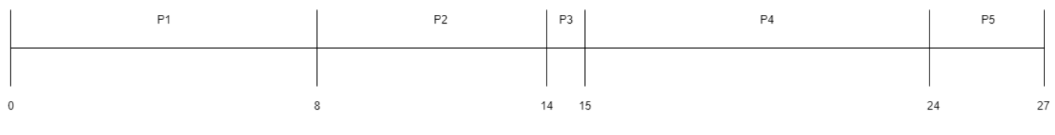
\includegraphics[width=17cm]{fcfs.png}
							\end{center}
						\end{figure}
					\item[$\bullet$] SJF:
						\begin{figure}[h!]
							\begin{center}
								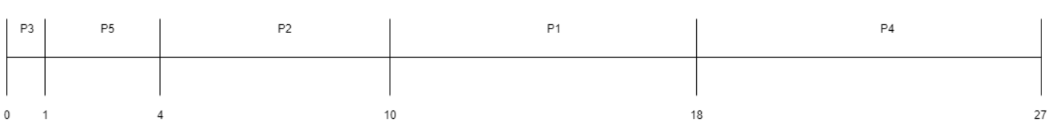
\includegraphics[width=17cm]{sjf.png}
							\end{center}
						\end{figure}
					\item[$\bullet$] Non-Preemptive Priority:
						\begin{figure}[h!]
							\begin{center}
								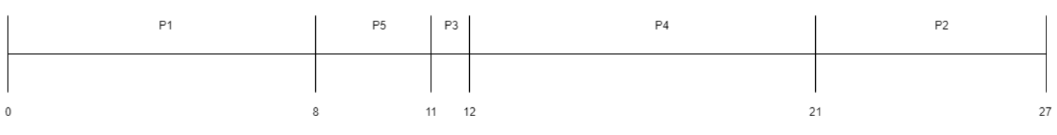
\includegraphics[width=17cm]{npp.png}
							\end{center}
						\end{figure}
					\item[$\bullet$] Round Robin (quantum = 1):
					\begin{figure}[h!]
						\begin{center}
							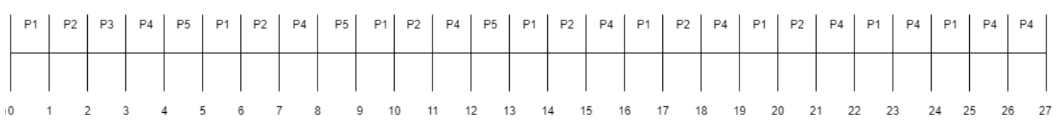
\includegraphics[width=17cm]{rr.png}
						\end{center}
					\end{figure}
				\end{enumerate}
			\item[$\circ$] \textbf{Average waiting time}
				\begin{center}
					\begin{tabular}{c|c|c|c|c}
						 & FCFS & SJF & Non-Preemptive Priority & Round Robin \\
						\hline
						P1 & $0$ & $10$ & $0$ & $17$ \\
						P2 & $8$ & $4$ & $21$ & $15$ \\
						P3 & $14$ & $0$ & $11$ & $2$ \\
						P4 & $15$ & $18$ & $12$ & $18$ \\
						P5 & $24$ & $1$ & $8$ & $10$ \\
						\hline
						Average Waiting Time & $12.2$ & $6.6$ & $10.4$ & $12.4$ \\
					\end{tabular}
				\end{center}
			\item[$\circ$] \textbf{Average turnaround time}
			\begin{center}
				\begin{tabular}{c|c|c|c|c}
					& FCFS & SJF & Non-Preemptive Priority & Round Robin \\
					\hline
					P1 & $8$ & $18$ & $8$ & $25$ \\
					P2 & $14$ & $10$ & $27$ & $21$ \\
					P3 & $15$ & $1$ & $12$ & $3$ \\
					P4 & $24$ & $27$ & $21$ & $27$ \\
					P5 & $27$ & $4$ & $11$ & $13$ \\
					\hline
					Average Turnaround Time & $17.6$ & $12.0$ & $15.8$ & $17.8$ \\
				\end{tabular}
			\end{center}
		\end{enumerate}
\end{document}